\documentclass[12pt]{article}
\usepackage[utf8]{inputenc}
\usepackage[english]{babel}
\usepackage{hyperref}
\usepackage{pdflscape}
\usepackage{enumitem}
\usepackage{makeidx}
\usepackage{csquotes}
\usepackage{chngcntr}

\usepackage{afterpage}
\usepackage{capt-of}
\usepackage{tikz}
\usepackage{pgfplots}
\usepackage{graphicx}
\graphicspath{ {./images/} }
\usepackage[acronym]{glossaries}
\usepackage[a4paper, inner=1.5cm, outer=3cm, top=2cm,bottom=3cm, bindingoffset=1cm]{geometry}
\counterwithin*{section}{part}
\usetikzlibrary{arrows.meta}
\usepackage{listings}
\usepackage{xcolor} 
\definecolor{codegreen}{rgb}{0,0.6,0}
\definecolor{codegray}{rgb}{0.5,0.5,0.5}
\definecolor{codepurple}{rgb}{0.58,0,0.82}
\definecolor{backcolour}{rgb}{0.95,0.95,0.92}
\tikzset{
  			>={Latex[width=2mm,length=2mm]},
            base/.style = {rectangle, rounded corners, draw=black,
                           minimum width=4cm, minimum height=1cm,
                           text centered, font=\sffamily},
  activityStarts/.style = {base, fill=blue!30},
       startstop/.style = {base, fill=red!30},
    activityRuns/.style = {base, fill=green!30},
         process/.style = {base, minimum width=2.5cm, fill=orange!15,
                           font=\ttfamily},
        }
        		
\begin{document}
\begin{titlepage}
    \begin{center}
        \vspace*{1cm} 
        \Huge
        \textbf{Comparative Approaches for Classification of Diabetes Mellitus Data} 
        \vspace{0.5cm}
        \normalsize
        \vspace{0cm}
        \\
        Study of machine learning algorithms and application on the Pima Indians Diabetes Dataset. 
        \vspace{1.5cm} 
        \\
        \textbf{Alexander Roque Rodrigues} 
        \vfill 
        A dissertation presented for the degree of\\
        Bachelor in Computer Science 
        \vspace{0.8cm}
        \Large        
        Department of Computer Science\\        
        Smt. Parvatibai Chowgule College of Arts and Science\\
        India\\
        18 August 2019 
    \end{center}
\end{titlepage}
\Huge
\newpage
\huge
\normalsize
\tableofcontents

\newpage
\part{Acknowledgements}
I, Alexander Roque Rodrigues, would like to acknowledge the role of the Department of Computer Science in guiding me and helping me to achieve the completion of this project. I would also like to acknowledge the efforts put in by my project guide Ms. Ashweta Fondekar, who assisted me throughout the span of the project and helped me achieve my goal. I also would like to thank my parents for their support and others who have indirectly assisted me in this project.


\newpage
\newlist{abbrv}{itemize}{1}
\setlist[abbrv,1]{label=,labelwidth=1in,align=parleft,itemsep=0.1\baselineskip,leftmargin=!}
 
\part{List of Abbreviations}
\begin{abbrv}
 
\item[T1D]			Type 1 Diabetes.
\item[T2D]			Type 2 Diabetes.
\item[GDM]			Gestational Diabetes.
\item[AEE]			Activity Energy Expenditure.
\item[CSII] 		Continuous Subcutaneous Insulin Infusion.
\item[MDI] 			Multiple Daily Injections.

\end{abbrv}

\newpage
\part{Introduction}
Data is everywhere. International initiatives coupled with global disruptive innovation are the leading causes for pushing datafication forward. Datafication refers to the modern-day trend of digitalizing (or datafying) every aspect of life. This data creation is enabling the transformation of data into new and potentially valuable forms. Entire municipalities are being incentivized to become smarter. In the not too distant future, our towns and cities will collect thousands of variables in real time to optimize, maintain, and enhance the quality of life for entire populations. One would reasonably expect that as well as managing traffic, traffic lights may also collect other data such as air quality, visibility, and speed of traffic. As a result of big data from connected devices, embedded sensors, and the IoT, there is a global need for the analysis, interpretation, and visualization of data.

\newpage
\part{Review of Literature}
\iffalse
Source : https://www.ncbi.nlm.nih.gov/pmc/articles/PMC5851210/
---------------------
Source : https://www.ncbi.nlm.nih.gov/pmc/articles/PMC6000484/
---------------------
PDF :
Andreas Holzinger 1,2( B )
Holzinger Group, HCI-KDD, Institute for Medical Informatics,
Statistics and Documentation, Medical University Graz, Graz, Austria
a.holzinger@hci-kdd.org

Institute for Information Systems and Computer Media,
Graz University of Technology, Graz, Austria
---------------------
\fi

There have been advances in the field of biotechnology along with easier and inexpensive methods of production of medical equipment has enabled easy production of data thereby allowing the generated big data to be used by machine learning algorithms.

To date, besides high performance sequencing methods, there is a plethora of digital machines and sensors from various research fields generating data, including super-resolution digital microscopy, mass spectrometry, Magnetic Resonance Imagery (MRI), etc. Although these technologies produce a wealth of data, they do not provide any kind of analysis, interpretation or extraction of knowledge. To this end, the area of Biological Data Mining or otherwise Knowledge Discovery in Biological Data, is more than ever necessary and important. The primary objective is to delve into the rapidly accruing body of biological data
and set the basis potentiating answers to fundamental questions in biology and medicine.

The power and effectiveness of these approaches are derived from the ability of commensurate methods to extract patterns and create
models from data. The aforementioned fact is particularly significant in the big data era, especially when the dataset can reach terabytes or petabytes of data. Consequently, the abundance of data has strengthened considerably data-oriented research in biology. In such a hybrid field, one of the most important research applications is prognosis and
diagnosis related to human-threatening and/or life quality reducing diseases. One such disease is diabetes mellitus (DM).

As defined by the American Diabetes Association\cite{classdiag},
\begin{quote}
Diabetes is a group of metabolic diseases characterized by hyperglycemia resulting from defects in insulin secretion, insulin action, or both. The chronic hyperglycemia of diabetes is associated with long-term damage, dysfunction, and failure of different organs, especially the eyes, kidneys, nerves, heart, and blood vessels.
\end{quote}


Diabetes Mellitus refers collectively to a group of diseases resulting from dysfunction of the glucoregulatory system. Hyperglycemia, the hallmark of diabetes, is the primary consequence of this dysregulation. Chronic hyperglycemia in diabetes is associated with long-term complications involving tissue damage and organ failure, which can decrease life expectancy and even cause death. The International Diabetes Federation estimates that, by 2017, diabetes affected 425 million people worldwide, of whom, 4 million died in the same year. These figures are expected to increase dramatically in the coming decades, placing a rising burden on health care systems. According to the growing morbidity in recent years, in 2040, the world’s diabetic patients will reach 642 million, which means that one of the ten adults in the future is suffering from diabetes. There is no doubt that this alarming figure needs great attention. With the rapid development of machine learning, machine learning has been applied to many aspects of medical health.\cite{DBTW}

Most diabetes cases can be categorized into 3 subgroups: 
\begin{enumerate}
\item T1D
\item T2D
\item GDM
\end{enumerate}

Over the long term, T2D patients become resistant to the normal effects of insulin and gradually lose their capacity to produce enough of this hormone. A wide range of therapeutic options are available for patients with T2D. At the early stages of disease, they commonly receive medications that improve insulin secretion or insulin absorption, but eventually they must receive external doses of insulin. On the other hand, T1D patients have severe impairments in insulin production, and must use external insulin exclusively to manage their blood glucose. Treatment of T1D requires consistent doses of insulin through MDI or CSII using a pump. GDM is treated similarly to T2D, but only occurs during pregnancy due to the interaction between insulin and hormones released by the placenta.

In each class of diabetes, timely diagnosis, education of patients in self-management, and continuous medical care are required to prevent acute complications (eg, ketoacidosis) and minimize the risk of long-term complications (eg, nephropathy, retinopathy, diabetic foot, cardiovascular disease, or stroke). In addition to medication, management of diabetes requires adherence to an array of self-care behaviors that are often very burdensome for patients: carefully scheduling meals, counting carbohydrates, exercising, monitoring BG levels, and adjusting endeavors on a daily basis. The effects of non-adherence to recommended treatment are not immediately evident and long-term complications may take years to develop. Accordingly, diabetes therapy is complex, and therapeutic decisions need to take into account diverse medical factors and lifestyle-related activities that must be optimized to improve diabetic patients’ quality of life.

Applying machine learning and data mining methods in diabetes mellitus research is a key approach to utilizing large volumes of available diabetes related data for extracting knowledge. The severe social impact of the specific disease renders DM one of the main priorities in medical science research, which inevitably generates huge amounts of data. Undoubtedly, therefore, machine learning and data mining approaches in DM are of great concern when it comes to diagnosis, management and other related clinical administration aspects. Hence, in the framework of this study, efforts were made to review the current literature on machine learning and data mining approaches in diabetes research.

Machine learning tasks are typically classified into three broad categories. These are: a) supervised learning, in which the system infers a function from labeled training data, b) unsupervised learning, in which the learning system tries to infer the structure of unlabeled data, and c) reinforcement learning, in which the system interacts with a dynamic environment.



\newpage
\part{Machine Learning Algorithms}
\section{Linear Regression}
Linear regression is a forecasting technique that can be use to predict the future of a number series based on the historic data given. The perks of using a linear regression model are as follows:

\begin{itemize}
  \item produces decent and  easy to interpret results.
  \item is computationally inexpensive.
  \item conversion of algorithm into code does not take much effort or time.
  \item numeric values as well as nominal values support is offered.
\end{itemize}

However, a major drawback of linear regression is that it \textbf{poorly models nonlinear data}.
\\
Considering a dataset that has values ranging from 
$X = \lbrace x_{1}+x_{2}+x_{3}+...+x_{n} \rbrace$ where
all the entries of the dataset are real numbers. Each $x_{i}$ is associated with a corresponding value of $y_{i}$ from the dataset $Y = \lbrace y_{1}+y_{2}+y_{3}+...+y_{n} \rbrace$.

The most basic equation for linear regression can be expressed via this simple equation.
$$y = \beta_{0}x+\beta_{1}+\epsilon$$

So to minimize the error in the predictions, a way to calculate the error should be formulated. A loss function in machine learning is simply a measure of how different the predicted value is from the actual value. The Quadratic Loss Function to calculate the loss or error in our linear regression model. It can be defined as:
$$L(x) = \sum_{i=1}^{n}(y_{i}-p_{i})^{2} $$
Therefore using the method of Least Squares, we can find the values of $\beta_{0}$ and $\beta_{1}$.

$$
\beta_{0} = \frac{\sum_{i=1}^{n} ( x_{i}-\bar{x}) (y_{i}-\bar{y})}{\sum_{i=1}^{n} ( x_{i}-\bar{x})^{2} }
$$
The linear regression model with an error value close to 1.00 indicates a perfect model and those with values closer to 0.00 indicates a model that delivers poor performance.



\newpage
\section{Logistic Regression}
Logistic Regression is a classification method which is based on the probability for a sample to belong to a class. As our probabilities must be continuous in $R$ and should bounded between the lower limit of 0 and upper limit of 1 it's necessary to introduce a threshold function to filter the term $z$. The name logistic comes from the decision to use the sigmoid (or logistic) function, defined as shown below.
$$\sigma(z)= \dfrac{1}{1+e^{-z}}$$
The sigmoid function in its domain is $R$ has two asymptotes\footnote{In analytic geometry, an asymptote of a curve is a line such that the distance between the curve and the line approaches zero as one or both of the x or y coordinates tends to infinity.} that occur at 0 and 1. So, the probability for a sample to belong to a class from 0 and 1 can be defined as:
$$P(y|\bar{x})=\sigma(\bar{x};\bar{w})$$
At this point, finding the optimal parameters is equivalent to maximizing the log-likelihood\footnote{The log-likelihood is, as the term suggests, the natural logarithm of the likelihood.}
given the output class:
$$L(\bar{w};y) = log P(y|\bar{w}) = \sum_{i} log P(y_{i}|\bar{x_{i}}, \bar{w})$$


\newpage
\section{K-Nearest Neighbours}
The k-means algorithm is based on the (strong) initial condition to decide the number of clusters through the assignment of k initial centroids or means:
% page 183
\\
Then the distance between each sample and each centroid is computed and the sample is
assigned to the cluster where the distance is minimum. This approach is often called
minimizing the inertia of the clusters, which is defined as follows:
%page 183
\\
The process is iterative—once all the samples have been processed, a new set of centroids K (1) is computed (now considering the actual elements belonging to the cluster), and all the distances are recomputed. The algorithm stops when the desired tolerance is reached, or in other words, when the centroids become stable and, therefore, the inertia is minimized. Of course, this approach is quite sensitive to the initial conditions, and some methods have been studied to improve the convergence speed. One of them is called k-means++ (Karteeka Pavan K., Allam Appa Rao, Dattatreya Rao A. V., and Sridhar G.R., Robust Seed Selection Algorithm for K-Means Type Algorithms, International Journal of Computer Science and Information Technology 3, no. 5, October 30, 2011), which selects the initial centroids so that they are statistically close to the final ones. The mathematical explanation is quite difficult; however, this method is the default choice for scikit-learn, and it's normally the best choice for any clustering problem solvable with this algorithm.
% page 188
\subsection{Finding Optimum Number of Clusters}
One of the most common disadvantages of k-means is related to the choice of the optimal number of clusters. An excessively small value will determine large groupings that contain heterogeneous elements, while a large number leads to a scenario where it can be difficult to identify the differences among clusters. Therefore, we're going to discuss some methods that can be employed to determine the appropriate number of splits and to evaluate the corresponding performance.

\subsection{Implementation}

\lstdefinestyle{mystyle}{
    backgroundcolor=\color{backcolour},   
    commentstyle=\color{codegreen},
    keywordstyle=\color{magenta},
    numberstyle=\tiny\color{codegray},
    stringstyle=\color{codepurple},
    basicstyle=\ttfamily\footnotesize,
    breakatwhitespace=false,         
    breaklines=true,                 
    captionpos=b,                    
    keepspaces=true,                 
    numbers=left,                    
    numbersep=5pt,                  
    showspaces=false,                
    showstringspaces=false,
    showtabs=false,                  
    tabsize=2
}
 
\lstset{style=mystyle}
\lstinputlisting[language=Python]{knn.py}



\newpage
\section{Decision Tree}
\subsection{Introduction}
Decision trees are flowcharts that represent the decision-making process as rules for performing categorization. Decision trees start from a root and contain internal nodes that represent features and branches that represent outcomes. As such, decision trees are a representation of a classification problem. Decision trees can be exploited to make them easier to understand. Each decision tree is a dis-junction of implications (i.e., if–then statements), and the implications are Horn clauses that are useful for logic programming. A Horn clause is a dis-junction of literals.
On the basis that there are no errors in the data in the form of inconsistencies, we can always construct a decision tree for training datasets with 100\% accuracy. However, this may not roll out in the real world and may indicate overfitting, as we will discuss.
\\
Classifying an example involves subjecting the data to an organized sequence of tests to determine the label. Trees are built and tested from top to bottom as so:

\begin{enumerate}
\item Start at the root of the model
\item Wait until all examples are in the same class
\item Test features to determine best split based on a cost function
\item Follow the branch value to the outcome
\item Repeat number 2
\item Leaf node output
\end{enumerate}

The central question in decision tree learning is which nodes should be placed in which positions, including the root node and decision nodes. There are three main decision tree algorithms. The difference in each algorithm is the measure or cost function for which nodes, or features, are selected. The root is the top node. The tree is split into branches; evaluated through a cost function; and a branch that doesn’t split is a terminal node, decision, or leaf.

Decision trees are useful in the way that acquired knowledge can be expressed in an easy to read and understandable format (see Figure 4-1). It mimics human decision-making whereby priority—determined by feature importance, relationships, and decisions—is clear. They are simple in the way that outcomes can be expressed as a set of rules. Figure 4-1. Decision tree of n = 2 nodes
Decision trees provide benefits in how they can represent big datasets and prioritize the most discriminatory features. If a decision tree depth is not set, it will eventually learn the data presented and overfit. It is recommended to set a small depth for decision tree modeling. Alternatively, the decision tree can be pruned, typically starting from the least important feature, or the incorporation of dimensionality reduction techniques.

Overfitting is a common machine learning obstacle, and not limited to decision trees. All algorithms are at risk of overfitting, and a variety of techniques exist to overcome this problem. Random forest or jungle decision trees can be extremely useful in this. Pruning reduces the size of a decision tree by removing features that provide the least information. As a result, the final classification rules are
less complicated and improve predictive accuracy. The accuracy of a model is calculated as the percentage of examples in
the test dataset that is classified correctly.

\begin{itemize}

\item{True Positive}: Where the actual class is yes, and
the value of the predicted class is also yes.

\item{False Positive}: Actual class is no, and predicted
class is yes.

\item{True Negative}: The value of the actual class is no,
and the value of the predicted class is no.

\item{False Negative}: When the actual class value is yes,
but predicted class is no.

\end{itemize}

$$
Accuracy= \frac{TP + TN}{TP + TN + FP + FN}
$$

$$
Precision = \frac{TP}{TP} + FP
$$

$$
Recall = \frac{TP}{TP} + FN
$$

Classification is a common method used in machine learning; and ID3 (Iterative Dichotomizer 3), C4.5 (Classification 4.5), and CART
(Classification And Regression Trees) are common decision tree methods where the resulting tree can be used to classify future samples.
\newpage
\section{Random Forest}

\newpage
\section{Gradient Boosting}

\newpage
\section{Support Vector Machine}
Support Vector Machines is an algorithm that is capable of handling 
linear as well as data that occurs non-linearly. For example, for a long time, SVMs were the best
choice for MNIST dataset classification, thanks to the fact that they can capture very high
non-linear dynamics using a mathematical trick, without complex modifications in the
algorithm.

\subsection{Linear Support Vector Machines}
Let us consider a dataset of features we want to classify.

$$
X = \lbrace x_{1}, x_{2}, x_{3}, ... , x_{n} \rbrace 
$$ 
For the target variable, we will consider the dataset $Y$, with target outcomes as 
$\lbrace0,1\rbrace$ indicating a true or false condition.

$$
Y = \lbrace y_{1}, y_{2}, y_{3}, ... , y_{n} \rbrace 
$$

\newpage
\section{Perceptron}

\newpage
\section{Multilayered Perceptron}

\newpage
\part{Real World Application}
This is the part on how the project results were obtained.\\


{%

    \clearpage% Flush earlier floats (otherwise order might not be correct)
    \thispagestyle{empty}% empty page style (?)
    \begin{landscape}% Landscape page
    \centering % Center table
\begin{table}[]
\begin{tabular}{|c|c|c|c|}
\hline
Algorithm              & Additional Parameters                              & Train Set Accuracy & Test Set Accuracy \\ \hline
K Nearest Neighbour    & -                                                  & 0.79               & 0.78              \\ \hline
Logistic Regression    & C = 1                                              & 0.781              & 0.771             \\ \hline
Logistic Regression    & C = 0.01                                           & 0.700              & 0.703             \\ \hline
Logistic Regression    & C = 100                                            & 0.785              & 0.766             \\ \hline
Decision Tree          & -                                                  & 1.00               & 0.714             \\ \hline
Decision Tree          & Max Depth = 3                                      & 0.773              & 0.740             \\ \hline
Random Forest          & Estimators = 100                                   & 1.000              & 0.786             \\ \hline
Random Forest          & Estimators = 100; Max Depth = 3                    & 0.800              & 0.755             \\ \hline
Gradient Boosting      & -                                                  & 0.917              & 0.792             \\ \hline
Gradient Boosting      & Max Depth = 1                                      & 0.804              & 0.781             \\ \hline
Gradient Boosting      & Learning Rate = 0.01                               & 0.802              & 0.776             \\ \hline
Support Vector Machine & -                                                  & 1.00               & 0.65              \\ \hline
Support Vector Machine & Train and Test set scaled using MinMaxScaler       & 0.77               & 0.77              \\ \hline
Support Vector Machine & C = 1000                                           & 0.790              & 0.797             \\ \hline
MLP Classifier         & Random State = 42                                  & 0.73               & 0.72              \\ \hline
MLP Classifier         & Random State = 0                                   & 0.823              & 0.802             \\ \hline
MLP Classifier         & Max Iterations = 1000                              & 0.908              & 0.792             \\ \hline
MLP Classifier         & Max Iterations = 1000; Alpha = 1; Random State = 0 & 0.806              & 0.797             \\ \hline
\end{tabular}
\end{table}
\captionof{table}{Test and Train accuracy's using various machine learning algorithms with various parameters.}% Add 'table' caption
    \end{landscape}
    \clearpage% Flush page
}



\newpage
\part{Building Information Systems for Prediction}
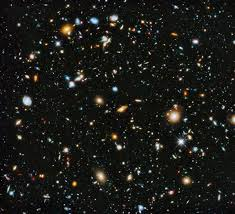
\includegraphics[width=\textwidth]{universe}
\section{Introduction}
In today's world we have many algorithms and multiple datasets along with sufficient data available for testing and training the algorithms for classifying whether or not a person from the healthy population has the risk of contracting diabetes or not. The system should be able to firstly mine the data or handle the incoming data and filter or process it according to the parameters described by the required specifications.


\section{Feature Selection}
\newpage
\section{Models}
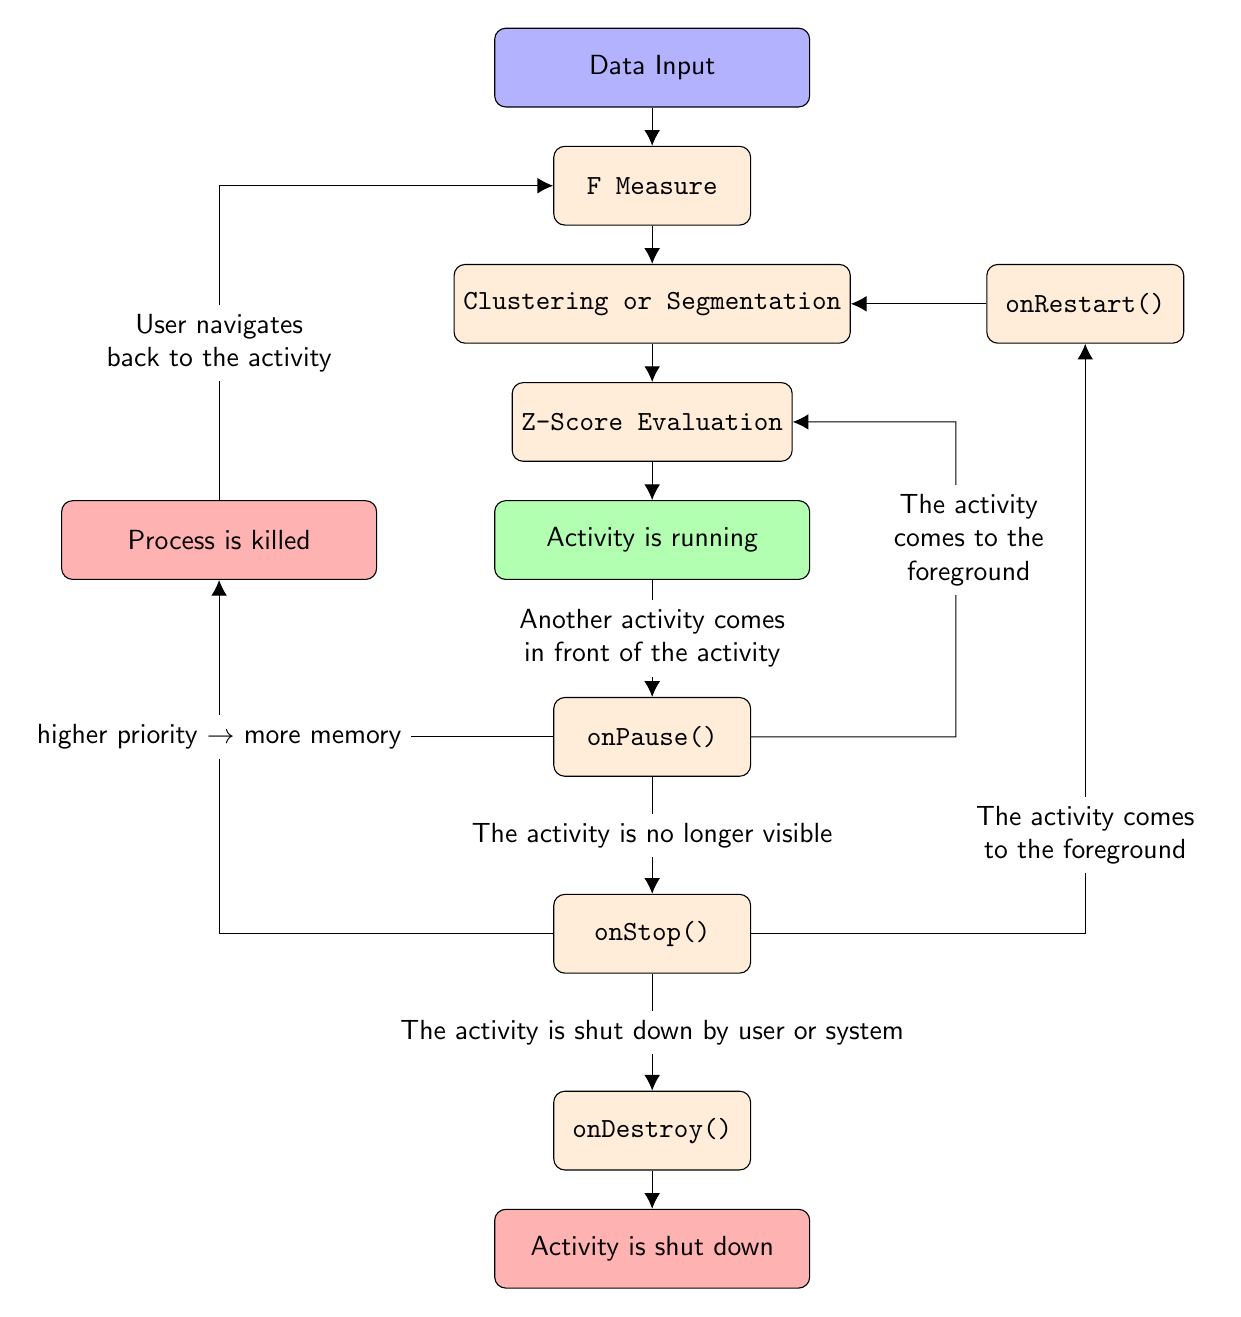
\begin{tikzpicture}[node distance=1.5cm,
    every node/.style={fill=white, font=\sffamily}, align=center]
  % Specification of nodes (position, etc.)
  \node (start)             [activityStarts]              {Data Input};
  \node (onCreateBlock)     [process, below of=start]          {F Measure};
  \node (onStartBlock)      [process, below of=onCreateBlock]   {Clustering or Segmentation};
  \node (onResumeBlock)     [process, below of=onStartBlock]   {Z-Score Evaluation};
  \node (activityRuns)      [activityRuns, below of=onResumeBlock]
                                                      {Activity is running};
  \node (onPauseBlock)      [process, below of=activityRuns, yshift=-1cm]
                                                                {onPause()};
  \node (onStopBlock)       [process, below of=onPauseBlock, yshift=-1cm]
                                                                 {onStop()};
  \node (onDestroyBlock)    [process, below of=onStopBlock, yshift=-1cm] 
                                                              {onDestroy()};
  \node (onRestartBlock)    [process, right of=onStartBlock, xshift=4cm]
                                                              {onRestart()};
  \node (ActivityEnds)      [startstop, left of=activityRuns, xshift=-4cm]
                                                        {Process is killed};
  \node (ActivityDestroyed) [startstop, below of=onDestroyBlock]
                                                    {Activity is shut down};     
  % Specification of lines between nodes specified above
  % with aditional nodes for description 
  \draw[->]             (start) -- (onCreateBlock);
  \draw[->]     (onCreateBlock) -- (onStartBlock);
  \draw[->]      (onStartBlock) -- (onResumeBlock);
  \draw[->]     (onResumeBlock) -- (activityRuns);
  \draw[->]      (activityRuns) -- node[text width=4cm]
                                   {Another activity comes in
                                    front of the activity} (onPauseBlock);
  \draw[->]      (onPauseBlock) -- node {The activity is no longer visible}
                                   (onStopBlock);
  \draw[->]       (onStopBlock) -- node {The activity is shut down by
                                   user or system} (onDestroyBlock);
  \draw[->]    (onRestartBlock) -- (onStartBlock);
  \draw[->]       (onStopBlock) -| node[yshift=1.25cm, text width=3cm]
                                   {The activity comes to the foreground}
                                   (onRestartBlock);
  \draw[->]    (onDestroyBlock) -- (ActivityDestroyed);
  \draw[->]      (onPauseBlock) -| node(priorityXMemory)
                                   {higher priority $\rightarrow$ more memory}
                                   (ActivityEnds);
  \draw           (onStopBlock) -| (priorityXMemory);
  \draw[->]     (ActivityEnds)  |- node [yshift=-2cm, text width=3.1cm]
                                    {User navigates back to the activity}
                                    (onCreateBlock);
  \draw[->] (onPauseBlock.east) -- ++(2.6,0) -- ++(0,2) -- ++(0,2) --                
     node[xshift=1.2cm,yshift=-1.5cm, text width=2.5cm]
     {The activity comes to the foreground}(onResumeBlock.east);
  \end{tikzpicture}

\newpage
\section{Conclusion}


\newpage
\part{Conclusion}

\clearpage
\newpage
\part{Bibliography}
\begin{thebibliography}{}
\bibitem{classdiag}
Diagnosis and Classification of Diabetes Mellitus. (2010). Retrieved November 28, 2019, from https://care.diabetesjournals.org/content/33/Supplement\_1/S62.

\bibitem{DBTW}
Home. (n.d.). Retrieved from https://www.idf.org/e-library/epidemiology-research/diabetes-atlas/134-idf-diabetes-atlas-8th-edition.html.

\bibitem{WMG} 
Wei M, Gibbons LW, Mitchell TL \textit{et al}. (1999) The Association between cardiorespiratory fitness and impaired fasting glucose and type 2 diabetes mellitus in men. \textit{Ann Intern Med} \textbf{130}, 427-34.

\bibitem{DEFD}
Jr., W. C. S. (2017, January 26). Definition of Diabetes mellitus. Retrieved November 17, 2019, from https://www.rxlist.com/script/main/art.asp?articlekey=2974.

\bibitem{DBML}
Zou, Q., Qu, K., Luo, Y., Yin, D., Ju, Y.,\& Tang, H. (2018, November 6). Predicting Diabetes Mellitus With Machine Learning Techniques. Retrieved November 17, 2019, from https://www.ncbi.nlm.nih.gov/pmc/articles/PMC6232260/.

\bibitem{WIKIUML}
Hinton, Geoffrey; Sejnowski, Terrence (1999). Unsupervised Learning: Foundations of Neural Computation. MIT Press. ISBN 978-0262581684.



\end{thebibliography}
\end{document}